\documentclass{ximera}
%  \input{../preamble.tex}
      
\title{MAT 151/111 (Precalculus/College Algebra) Activity}
      
\begin{document}
      
\begin{abstract}
      
Some sample questions that can be related to MAT 111 (College Algebra) or 151 (Precalculus).
      
\end{abstract}
      
\maketitle
      
      
      
\begin{question}
      
  What type of function best describes $f(t)=7\cdot\left(\frac{2}{3}\right)^t$?
      
  \begin{multipleChoice}
      
    \choice{linear}
      
    \choice{quadratic}
    
    \choice{polynomial}
    \choice{rational}
    \choice[correct]{exponential}
    \choice{trigonometric}
    \choice{inverse trigonometric}
          
  \end{multipleChoice}
      
\end{question}      

\begin{question}
What is $\cos^{-1}(-1)$ in radians?
\begin{explanation}

Consider the unit circle:

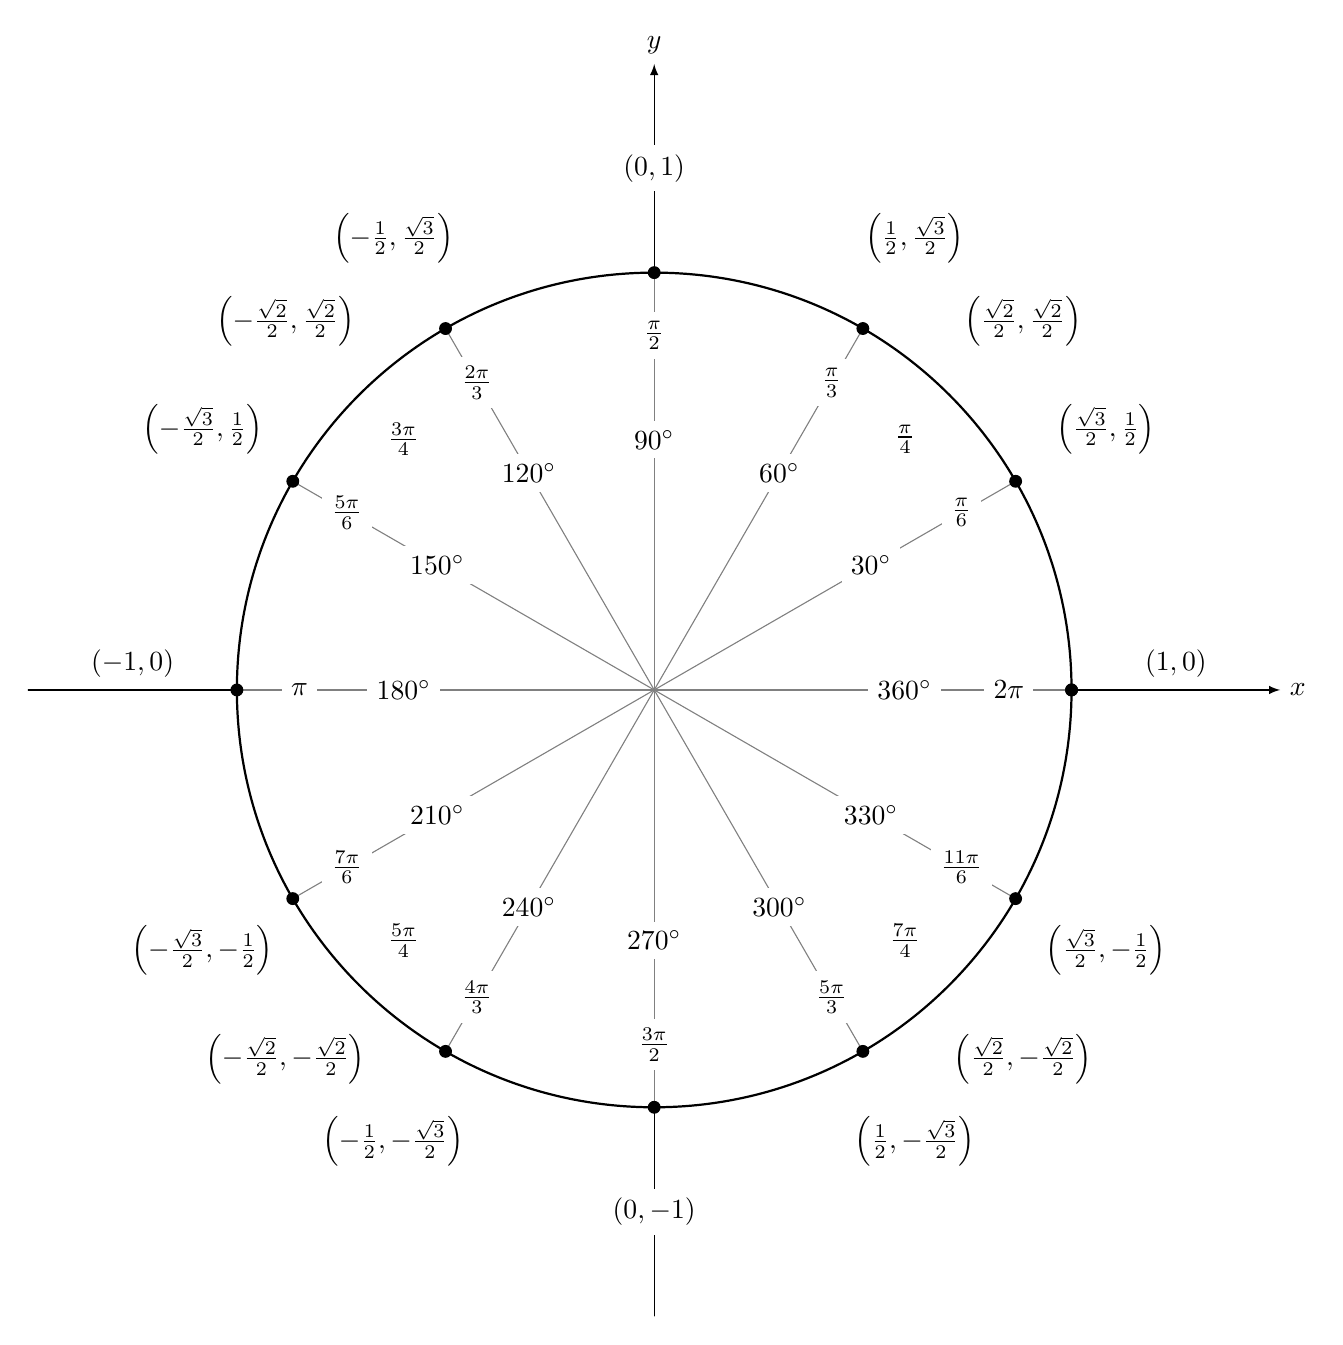
\begin{tikzpicture}[scale=5.3,cap=round,>=latex]
        % draw the coordinates
        \draw[->] (-1.5cm,0cm) -- (1.5cm,0cm) node[right,fill=white] {$x$};
        \draw[->] (0cm,-1.5cm) -- (0cm,1.5cm) node[above,fill=white] {$y$};

        % draw the unit circle
        \draw[thick] (0cm,0cm) circle(1cm);

        \foreach \x in {0,30,...,360} {
                % lines from center to point
                \draw[gray] (0cm,0cm) -- (\x:1cm);
                % dots at each point
                \filldraw[black] (\x:1cm) circle(0.4pt);
                % draw each angle in degrees
                \draw (\x:0.6cm) node[fill=white] {$\x^\circ$};
        }

        % draw each angle in radians
        \foreach \x/\xtext in {
            30/\frac{\pi}{6},
            45/\frac{\pi}{4},
            60/\frac{\pi}{3},
            90/\frac{\pi}{2},
            120/\frac{2\pi}{3},
            135/\frac{3\pi}{4},
            150/\frac{5\pi}{6},
            180/\pi,
            210/\frac{7\pi}{6},
            225/\frac{5\pi}{4},
            240/\frac{4\pi}{3},
            270/\frac{3\pi}{2},
            300/\frac{5\pi}{3},
            315/\frac{7\pi}{4},
            330/\frac{11\pi}{6},
            360/2\pi}
                \draw (\x:0.85cm) node[fill=white] {$\xtext$};

        \foreach \x/\xtext/\y in {
            % the coordinates for the first quadrant
            30/\frac{\sqrt{3}}{2}/\frac{1}{2},
            45/\frac{\sqrt{2}}{2}/\frac{\sqrt{2}}{2},
            60/\frac{1}{2}/\frac{\sqrt{3}}{2},
            % the coordinates for the second quadrant
            150/-\frac{\sqrt{3}}{2}/\frac{1}{2},
            135/-\frac{\sqrt{2}}{2}/\frac{\sqrt{2}}{2},
            120/-\frac{1}{2}/\frac{\sqrt{3}}{2},
            % the coordinates for the third quadrant
            210/-\frac{\sqrt{3}}{2}/-\frac{1}{2},
            225/-\frac{\sqrt{2}}{2}/-\frac{\sqrt{2}}{2},
            240/-\frac{1}{2}/-\frac{\sqrt{3}}{2},
            % the coordinates for the fourth quadrant
            330/\frac{\sqrt{3}}{2}/-\frac{1}{2},
            315/\frac{\sqrt{2}}{2}/-\frac{\sqrt{2}}{2},
            300/\frac{1}{2}/-\frac{\sqrt{3}}{2}}
                \draw (\x:1.25cm) node[fill=white] {$\left(\xtext,\y\right)$};

        % draw the horizontal and vertical coordinates
        % the placement is better this way
        \draw (-1.25cm,0cm) node[above=1pt] {$(-1,0)$}
              (1.25cm,0cm)  node[above=1pt] {$(1,0)$}
              (0cm,-1.25cm) node[fill=white] {$(0,-1)$}
              (0cm,1.25cm)  node[fill=white] {$(0,1)$};
    \end{tikzpicture}

Now, given any angle $\theta$, we have that $\sin(\theta)$ corresponds to the:

\begin{multipleChoice}
\choice{$x$ coordinate.}
\choice[correct]{$y$ coordinate.}
\end{multipleChoice}
Similarly, $\cos(\theta)$ corresponds to the:
\begin{multipleChoice}
\choice[correct]{$x$ coordinate.}
\choice{$y$ coordinate.}
\end{multipleChoice}

So given the variable corresponding to $\theta$, that variable has value $-1$ exactly once on the unit circle, and that occurs when $\theta=\answer{\pi}$.  Thus $\cos^{-1}(-1)=\answer{\pi}$.


\end{explanation}
\end{question}

\begin{question}
Consider the line $y=3x+4$

\begin{enumerate}
\item The slope of the line is $m=\answer[]{3}$.
\item The $y$ intercept occurs when $y=\answer[]{4}$.
\item The $x$ intercept occurs when $x=\answer[]{-4/3}$.
\item  If $x$ represents a number of tons of bubblegum, and $y$ in thousands of dollars the cost of manufacturing $x$ tons of bubblegum,  If one had \$20,000, how much bubblegum could you manufacture?\\ \\

So, we are told information about the $y$ value, and this is because:

\begin{multipleChoice}
\choice{We know how much bubblegum to make.}
\choice[correct]{We know how much money to spend.}
\end{multipleChoice}

So the given value for $y$ is $y=\answer{20}$.  This gives the equation:

\begin{eqnarray*}
\answer{20}&=&3x+4\\
\answer{16}&=&3x\\
\answer{16/3}&=&x\\
\end{eqnarray*}

So we could make $\answer{16/3}$ tons of bubblegum.

\item The line perpendicular to this line with $x$ intercept $(6,0)$ is   $y=\answer[]{-x/3+2}$.
\end{enumerate}


\end{question}



\begin{question}

To derive a general formula for the solutions to $ax^2+bx+c=0$, consider the following:

\begin{eqnarray*}
ax^2+bx+c&=& 0\\
0&=&a(x^2+\answer[]{\frac{b}{a}}x)+c,\ \text{by factoring out the $a$} \\
0&=& a(x^2+\answer[]{\frac{b}{a}}x+\answer[]{\frac{b^2}{4a^2}}-\answer[]{\frac{b^2}{4a^2}})+c, \\ 
&&\text{by completing the square.}\\
0&=&a(x^2+\answer[]{\frac{b}{a}}x+\answer[]{\frac{b^2}{4a^2}})-\answer[]{\frac{b^2}{4a}}+c,\\
 && \text{by distribution.}\\
0&=&a(x+\answer[]{\frac{b}{2a}})^2-\answer[]{\frac{b^2}{4a}}+c,\\
&&\text{by factoring}\\
0&=&a(x+\answer[]{\frac{b}{2a}})^2+\answer[]{\frac{b^2-4ac}{4a}},\\
&& \text{by finding common denominator and finessing the negative}\\
-\answer[]{\frac{b^2-4ac}{4a}}&=&a(x+\answer[]{\frac{b}{2a}})^2, \\
&& \text{subtract from both sides}\\
-\answer[]{\frac{b^2-4ac}{4a^2}}&=&(x+\answer[]{\frac{b}{2a}})^2, \\
&& \text{divide both sides}\\
-\frac{\pm \sqrt{\answer[]{b^2-4ac}}}{\answer[]{2a}}&=&x+\answer[]{\frac{b}{2a}}\\
&& \text{taking square roots of both sides}\\
x&=&\frac{-\answer[]{b}\pm \sqrt{\answer[]{b^2-4ac}}}{\answer[]{2a}}.\\
&& \text{by subtracting from both sides and simplifying.}
\end{eqnarray*}


\end{question}


%\begin{question}
%
% \begin{onlineOnly}
%   Consider the graph $y=f(x)$:
%   \[
%   \graph[xmin=0,xmax=10,ymin=-10,ymax=10]{y=x\left\{x<2\right\},y=-x^2+6\left\{2\leq x<4\right\},y=3x-22\left\{3 \leq x\right\}} 
%   \]
% \end{onlineOnly}
%
%\begin{enumerate}
%\item The $y$ intercept of this graph is $(\answer[]{0},0)$.
%\item If this graph represents the profits of a company in week $x$ of operation in thousands of dollars per week, then in when is the profitability of the company $\$5000/$week?  In week $\answer[]{9}$.
%\end{enumerate}
%
%
%
%\end{question}


\begin{question}
Consider the graph of the function $f(x)=\begin{cases}   x & -3\leq x \leq -1 \\ 3x+2 &-1<x<0 \\ 2 & 0\leq x\leq 2\end{cases}.$

 \begin{onlineOnly}
   \[
   \graph[xmin=-4,xmax=4,ymin=-4,ymax=4, panel]{y=x\left\{-3\leq x\leq -1\right\},y=-3x+2\left\{-1<x<0\right\},y=2\left\{0 \leq x\leq 2\right\}} 
   \]
 \end{onlineOnly}
(The above Desmos graph shows the graph of $f(x)$ as described above.  The link \url{https://www.desmos.com/calculator/zmsp6bcsiq} displays a graph for $g(x):=bf(ax+h)+k$.  Sliders for $a,b,k,h$ control the graph of $g(x)$, allowing for displays of multiple transformations of $y=f(x)$.)


\begin{enumerate}
\item Find the domain and range of $f(x)$.\\ \\ From the graph above or from the definition of $f(x)$, the smallest value for which $f(x)$ is defined is $\answer{-3}$.  Similarly, the largest value for which it is defined is $\answer{2}$.  Thus the domain of $f(x)$ is $[\answer{-3}, \answer{2}]$.  By taking the same observation of the outputs of $f(x)$, the range is $[\answer{-3}, \answer{2}]$.

\item Consider $g(x)=f(x+2)$
\begin{enumerate}
\item What is $g(-1)$?  \\ \\ Notice that $g(-1)=f(-1+\answer{2})=f(\answer{1})$.  By observing the graph above, we notice that $g(-1)=f(\answer{1})=\answer{2}$.  Similarly, if we observe that we are evaluating $f$ in the region:

\begin{multipleChoice}
\choice{$-3\leq x\leq-1$}
\choice{$-1<x<0$}
\choice[correct]{$0\leq x\leq 2$}
\end{multipleChoice}

So for our problem, $f(\answer{1})=\answer{2}$.

\item Similarly $g(-5)=\answer{-3}$ and $g(0)=\answer{2}$

\item Use the sliders in the link to observe the graph of $f(x)$.  The parameters should be $a=\answer{1}, b=\answer{1}, h=\answer{2}, k=\answer{0}$.

\item The domain of $g(x)$ is $[\answer{-5}, \answer{0}]$ and the range is $[\answer{-3}, \answer{2}]$.

\end{enumerate}


\item Consider $h(x)=-2f(x)$
\begin{enumerate}
\item What is $h(-1)$?  \\ \\ Notice that $h(-1)=\answer{-2}\cdot f(-1)$.  By observing the graph above, we notice that $h(-1)=\answer{-2}\cdot f(-1)=\answer{2}$.  Note that we are evaluating $f$ in the region:

\begin{multipleChoice}
\choice[correct]{$-3\leq x\leq-1$}
\choice{$-1<x<0$}
\choice{$0\leq x\leq 2$}
\end{multipleChoice}

So for our problem, $\answer{-2}\cdot f(-1)=\answer{2}$.

\item Similarly $h(2)=\answer{-4}$ and $h(-0.5)=\answer{-1}$

\item Use the sliders in the link to observe the graph of $f(x)$.  The parameters should be $a=\answer{1}, b=\answer{-2}, h=\answer{0}, k=\answer{0}$.

\item The domain of $g(x)$ is $[\answer{-3}, \answer{2}]$ and the range is $[\answer{6}, \answer{-4}]$.

\end{enumerate}





\end{enumerate}

\end{question}



\end{document}
